%!TEX root = proposal.tex
\chapter{Research Objectives and Approach}
\label{ch:plan}


%%%%%%%%%%%%%%%%%%%%%%%%%%%%%%%%%%%%%%%%%%%%%%%%%%%%%%%%%%%%%%%%%%%%%%%%%%%%%%%
%%%%%%%%%%%%%%%%%%%%%%%%%%%%%%%%%%%%%%%%%%%%%%%%%%%%%%%%%%%%%%%%%%%%%%%%%%%%%%%
\textcolor{blue}{The chapter Research Objectives and Approach clarifies the research objectives of your 
project, taking as its background your description of the state of the art, and describes 
the methodological approaches you have in mind to face the key research challenges of 
your project. The clarification of the research objectives should build solidly on the 
State of the Art and relate your research to the work carried out by others. It should 
elucidate the measure to which your work develops from their work and the extent to 
which it diverges from theirs to open up new and yet unexplored avenues. In essence, 
the chapter Research Objectives and Approach explains what you plan to do to tackle 
your research problem, why you plan to do it that way, and how you are going to do it.  
The “how to” component of the proposal is called the Research Methods, or 
Methodology, component. It should be detailed enough to let the reader decide whether 
the methods you intend to use are adequate for the research at hand. It should go beyond 
the mere listing of research tasks, by asserting why you assume that the methods or 
methodologies you have chosen represent the best available approaches for your project. 
This means that you should include a discussion of possible alternatives and credible 
explanations of why your approach is the most valid. }
% %%%%%%%%%%%%%%%%%%%%%%%%%%%%%%%%%%%%%%%%%%%%%%%%%%%%%%%%%%%%%%%%%%%%%%%%%%%%%%%
% %%%%%%%%%%%%%%%%%%%%%%%%%%%%%%%%%%%%%%%%%%%%%%%%%%%%%%%%%%%%%%%%%%%%%%%%%%%%%%%


\section{Expected impact}
\label{sec:impact}



%% Workplan 
\section{Work Plan} 
\label{sec:workplan}





%%%%%%%%%%%%%%%%%%%%%%%%%%%%%%%%%%%%%%%%%%%%%%%%%%%%%%%%%%%%%%%%%%%%%%%%%%%%%%%
%%%%%%%%%%%%%%%%%%%%%%%%%%%%%%%%%%%%%%%%%%%%%%%%%%%%%%%%%%%%%%%%%%%%%%%%%%%%%%%
\textcolor{blue}{
Not all research proposals lend themselves easily to the creation of detailed work plans. 
In some cases, namely when the work fits the broader plans of a research group that is 
progressing steadily, it is possible do build a detailed description of what the researcher 
plans to do (literature to explore in depth, principles or theorems to formulate and 
prove, experiments to carry out, sub-systems to build, systems integrations to perform, 
tests to accomplish). In these cases, it is possible, and desirable, to establish specific 
milestones and timelines and a Gantt diagram. The plan should anticipate the problems 
likely to be found along the way and describe the approaches to be followed in solving 
them. It should also anticipate the conferences and journals to which the work in 
progress is expected to be submitted along the way, and schedule it in a Goals for 
Publication section of the work plan. 
In other cases, when the topic to be researched is exploratory and elusive, or when the 
research approach establishes that each step should build on the, still unanticipated, 
results of previous steps, it may be impossible to work out a detailed plan. Even in these 
cases, however, it is advisable to establish a section on Goals for Publications that gives 
a rough schedule of the publications to be produced (submission to the doctoral 
consortium of a top conference, submission to a national conference, publication in a 
secondary journal, submission to a reputable international conference, submission to the 
top conference or top journal in the field). In spite of its contingency, this list may work 
marvels in keeping the researcher focused, motivated and beneficially under pressure. 
Table \ref{tab:plan} shows my plan for completion of the research.}


% compile timeline_teste.tex
\begin{landscape}
	\begin{figure}
	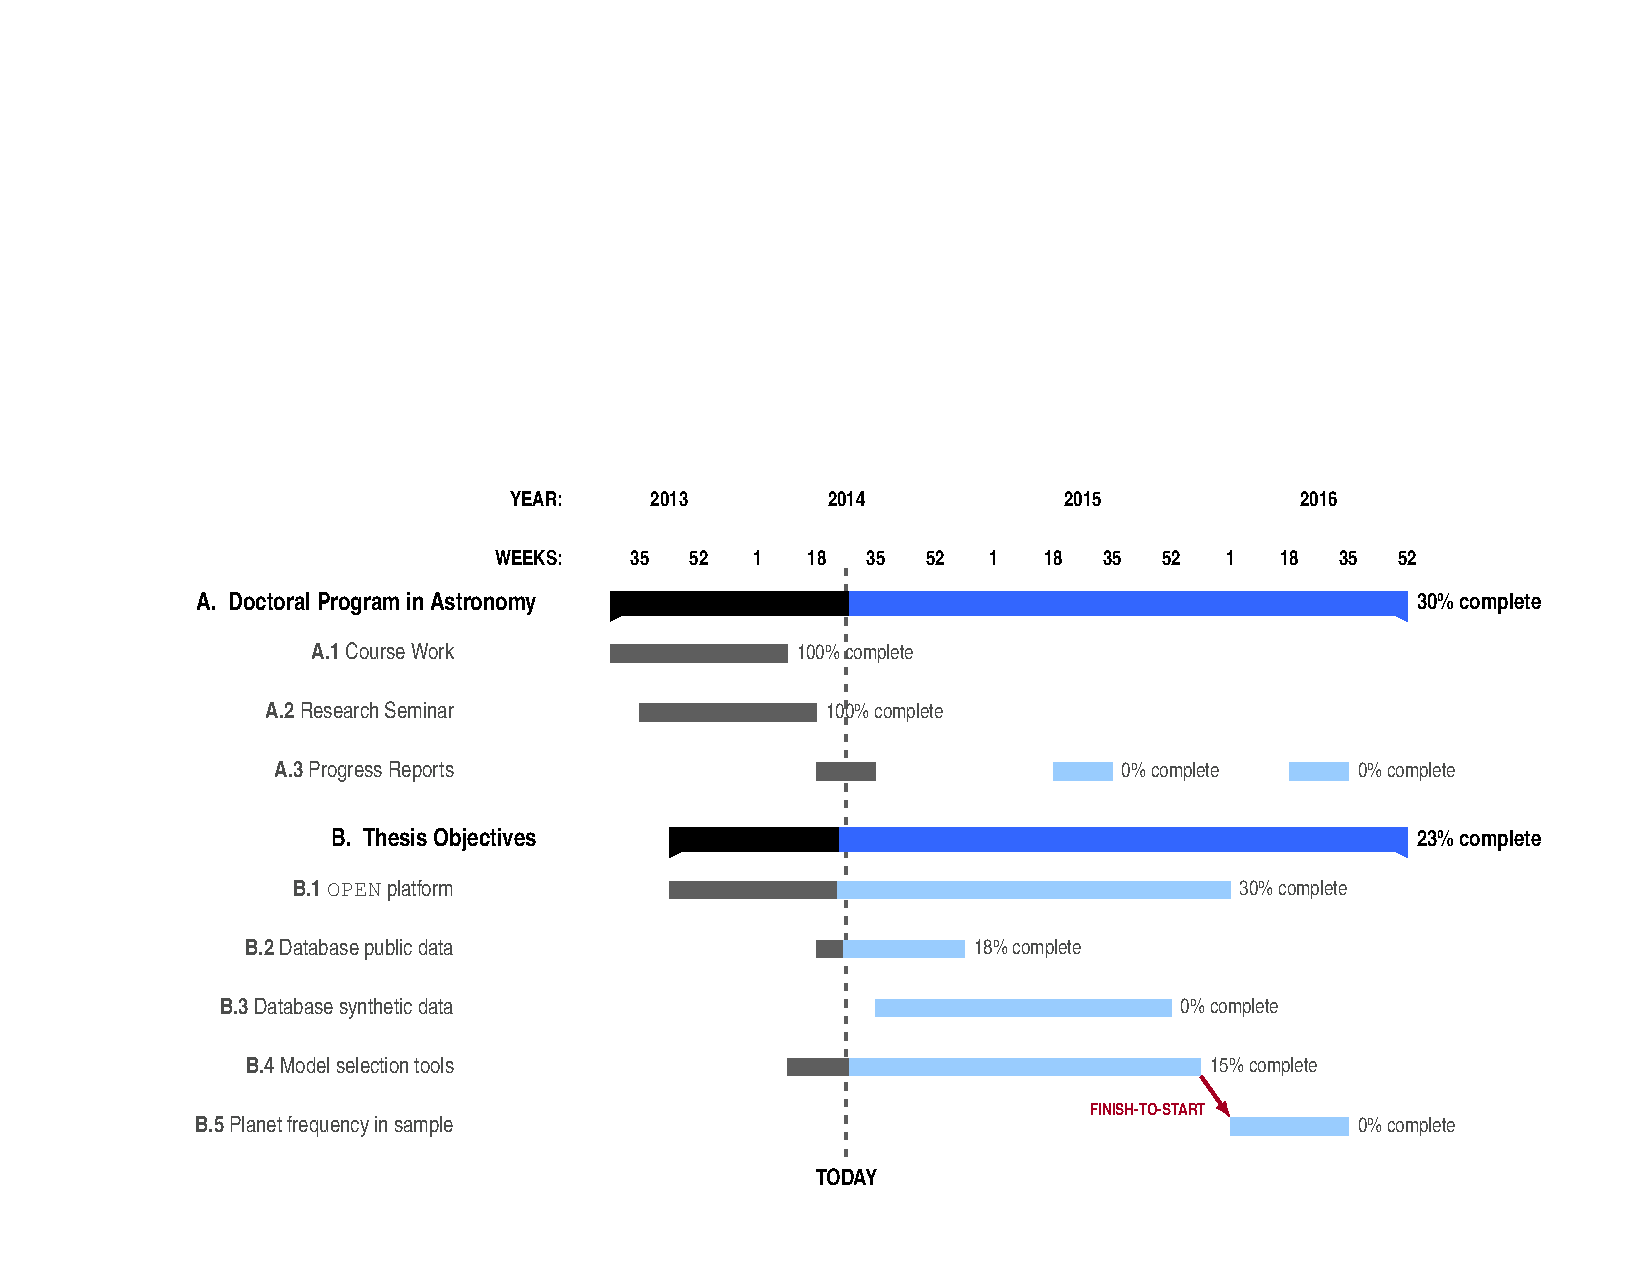
\includegraphics[trim=75 0 0 200, clip]{./timeline_teste.pdf}
	\sscaption{%
	\label{fig:ganttchart}}
	\end{figure}
\end{landscape}